\documentclass[review]{elsarticle}

\usepackage{lineno,hyperref}
\usepackage{eurosym}
\modulolinenumbers[5]

\journal{Journal of \LaTeX\ Templates}

% wording
\newcommand {\ie}{\mbox{i.e.}\xspace}     %i.e.
\newcommand {\eg}{\mbox{e.g.}\xspace}     %e.g.

% formulas
\newcommand{\fe}{\ensuremath{^{55}\textrm{Fe}}\xspace}
\newcommand{\abs}[1]{\ensuremath{\vert #1 \vert}}
\newcommand{\ambe}{\ensuremath{\textrm{Am} \textrm{Be}}\xspace}
\newcommand{\isclu}{\ensuremath{I_{SC}}\xspace}

% detector and algorithms
\newcommand{\lemon}{{\textsc{Lemon}}\xspace}
\newcommand{\idbscan}{{\textsc{iDbscan}}\xspace}
\newcommand{\dbscan}{{\textsc{Dbscan}}\xspace}
\newcommand{\gac}{{\textsc{Gac}}\xspace}
\newcommand{\nnc}{{\textsc{Nnc}}\xspace}
\newcommand{\GEANT} {{\textsc{Geant4}}\xspace}
\newcommand{\SRIM} {{\textsc{Srim}}\xspace}
\newcommand{\garfield} {{\textsc{Garfield}}\xspace}

% units
\newcommand{\unit}[1]{\ensuremath{\textrm{\,#1}}\xspace}
\newcommand{\keV}{\ensuremath{\,\textrm{ke\hspace{-.08em}V}}\xspace}

% GEM stuff
\newcommand{\Itot}{I$_{\mathrm{Tot}}$\xspace}
\newcommand{\Ig}  {I$_{\mathrm{G3U}}$\xspace}
\newcommand{\Ed}  {E$_{\mathrm{D}}$\xspace}
\newcommand{\Et}  {E$_{\mathrm{Transf}}$\xspace}
\newcommand{\Vg}  {V$_{\mathrm{GEM}}$\xspace}
\newcommand{\Dt}  {$D_{\mathrm{T}}$\xspace}
\newcommand{\Dl}  {$D_{\mathrm{L}}$\xspace}

%%%%%%%%%%%%%%%%%%%%%%%
%% Elsevier bibliography styles
%%%%%%%%%%%%%%%%%%%%%%%
%% To change the style, put a % in front of the second line of the current style and
%% remove the % from the second line of the style you would like to use.
%%%%%%%%%%%%%%%%%%%%%%%

%% Numbered
%\bibliographystyle{model1-num-names}

%% Numbered without titles
%\bibliographystyle{model1a-num-names}

%% Harvard
%\bibliographystyle{model2-names.bst}\biboptions{authoryear}

%% Vancouver numbered
%\usepackage{numcompress}\bibliographystyle{model3-num-names}

%% Vancouver name/year
%\usepackage{numcompress}\bibliographystyle{model4-names}\biboptions{authoryear}

%% APA style
%\bibliographystyle{model5-names}\biboptions{authoryear}

%% AMA style
%\usepackage{numcompress}\bibliographystyle{model6-num-names}

%% `Elsevier LaTeX' style
\bibliographystyle{elsarticle-num}
%%%%%%%%%%%%%%%%%%%%%%%

\begin{document}

\begin{frontmatter}

\title{The CYGNO Experiment}

%% Group authors per address:
 

%\author{Elsevier\fnref{myfootnote}}
%\address{Radarweg 29, Amsterdam}
%\fntext[myfootnote]{Since 1880.}

%% or include addresss in footnotes:

\author[a,b]{E. Baracchini,} 
\author[c]{R Bedogni,} 
\author[e,f]{F Bellini,} 
\author[c]{L. Benussi,}
\author[c]{S. Bianco,}
\author[c]{C. Capoccia,} 
\author[c,d]{M. Caponero,}
\author[e,f]{G. Cavoto,}
\author[a,b]{A. Cortez,}
\author[g]{I. A. Costa,}
\author[e]{E. Di Marco,}
\author[e]{G. D'Imperio,}
\author[a,b]{G. Dho,}
\author[e]{F. Iacoangeli,}
\author[c]{G. Maccarrone,}
\author[e,h]{M. Marafini,}
\author[c]{G. Mazzitelli,}
\author[e,f]{A. Messina,}
\author[g]{R. A. Nobrega,}
\author[c]{A. Orlandi,}
\author[c]{E. Paoletti,}
\author[c]{L. Passamonti,}
\author[i,j]{F. Petrucci,}
\author[c]{D. Piccolo,}
\author[c]{D. Pierluigi,}
\author[e]{D. Pinci\corref{mycorrespondingauthor}}
\author[e]{F. Renga,}
\author[c]{F. Rosatelli,}
\author[c]{A. Russo,}
\author[c,k]{G. Saviano,}
\author[c]{and S. Tomassini}

\cortext[mycorrespondingauthor]{Corresponding author}

\address[a]{Gran~Sasso~Science~Institute,\\ L'Aquila, I-67100, Italy}
\address[b]{Istituto Nazionale di Fisica Nucleare,\\ Laboratori Nazionali del Gran Sasso, Assergi, Italy}
\address[c]{Istituto Nazionale di Fisica Nucleare ,\\  Laboratori Nazionali di Frascati, I-00044, Italy}
\address[d]{ENEA Centro Ricerche Frascati, Frascati, Italy}
\address[e]{Istituto~Nazionale~di~Fisica~Nucleare,\\ Sezione di Roma, I-00185, Italy}
\address[f]{Dipartimento di Fisica Sapienza Universit\`a di Roma, I-00185, Italy} 
\address[g]{Universidade Federal de Juiz de Fora, Juiz de Fora, Brasil}
\address[h]{Museo Storico della Fisica e Centro Studi e Ricerche "Enrico Fermi",\\ Piazza del Viminale 1, Roma, I-00184, Italy}
\address[i]{Dipartimento di Matematica e Fisica, Universit\`a Roma TRE, Roma, Italy}
\address[j]{Istituto Nazionale di Fisica Nucleare, Sezione di Roma TRE, Roma, Italy}
\address[k]{Dipartimento di Ingegneria Chimica, Materiali e Ambiente, Sapienza Universit\`a di Roma, Roma, Italy}


\begin{abstract}
The search for a novel technology able to detect and reconstruct nuclear recoil events in the \keV energy range has become more and more important as long as vast regions of high mass WIMP-like Dark Matter candidate have been excluded.
Gaseous Time Projection Chambers (TPC) with optical readout are very promising candidate combining the complete event information provided by TPC technique to the high sensitivity and granularity of last generation scientific light sensors.
CYGNO (a CYGNUs module with Optical readout) is an experiment that aims at searching Dark Matter in the low mass region, exploiting very promising performance of the Optical Readout approach of multiple-GEM structures for large volume TPC. 
This experiment is part the CYGNUS proto-collaboration which aims at constructing a network of underground observatories
for directional Dark Matter search. 
The combined use of high-granularity sCMOS and
fast sensors to read out the light allows the reconstruction of the 3D direction of the tracks, offering good energy resolution and very high sensitivity in the keV energy range together with a very good particle identification useful to distinguish nuclear recoils from electronic
recoils. A 1 cubic meter demonstrator is expected to be built in 2020/21 aiming to a larger scale apparatus (30m$^3$-100 m$^3$), 
in a later stage.
\end{abstract}

\begin{keyword}
%\texttt{elsarticle.cls}\sep \LaTeX\sep Elsevier \sep template
%\MSC[2010] 00-01\sep  99-00
\end{keyword}

\end{frontmatter}

\linenumbers

\section{Introduction}
\section{The CYGNO project}

The aim of CYGNO project is the development and realisation of a GEM-based Optically Readout Time Projection Chamber for the study of rare events with energy releases in the range 1-100~keV. 

As it will be described in this paper, such a technology will allow the study of possible Dark Matter signals in mass regions still un-explored together with the possibility of 

A gas represents an interesting target: nuclei free paths can be long enough to be reconstructed. 
In particular, $\epsilon$ the maximum fraction of the energy that can be
transferred to the nucleus of mass $m_N$ by a Dark Matter particle of mass
$m_{\chi}$ is given by:
\begin{equation}
\epsilon = \frac {4 \rho}{\left( \rho + 1 \right)^2}
\label{eq:trans}
\end{equation}

where $\rho = \frac{m_N}{m_{\chi}}$.


\section{The Optical Readout Approach}
\label{sect:opro}

In recent years different groups started working on the development of optical readout of gas detectors (citazioni). In particular, very interesting results were obtained when CMOS-based sensors were employed for the acquisition of Time Projection Chambers (TPC) equipped with multiplication stages based on Micro-Pattern Gas Detectors (MPDG) (citazioni).

Main limitation in the development of this technique was represented
by the low signal/noise ratio of the light sensors. Mainly CCD have being
used in past with a noise of 5$\div$10 photons/pixel. This, allowed to
detect only highly ionizing particle tracks.

CYGNO collaboration first proposed the use of CMOS based optical device, 
for GEM-based detector optical readout \cite{bib:orange1, bib:orange2, bib:orange3, bib:orange4, bib:elba}.


High-granularity and low-noise image sensors in CMOS technology offer high level performance. State-of-the-art imagers contain tens of millions of pixels, with very low dark current (down to 2 e-/s/pixel), sub-electron readout noise and high sensitivity, so that they provide almost single photon detection. 

On the other hand, MPDG production technology guarantees very high quality devices, providing stable and uniform operation.

Time projection chambers, developed for high-energy experiment, provide the possible of collecting a complete and useful set of information about events:
\begin{itemize}
    \item it is possible to make a 3D reconstruction of the tracks in sensitive volume;
    \item it can evaluate not only the total amount of released energy, but also its profile along the particle trajectory allowing to reconstruct the dE/dx, very helpful for particle identification and track head-tail discrimination;
    \item large volumes can be acquired with small amount of readout channels. 
\end{itemize}

For equipping large surfaces, the use of Micro Pattern Gas Detectors
is a very simple solution ensuring high space and time resolution.
In particular Gas Electron Multipliers are able to suppress
the Ion Back Flow inside the sensitive volume. 

The optical readout approach has several advantages:
\begin{itemize}
\item sensors can be installed  outside the 
sensitive volume reducing the interference with  the GEM high voltage operation and reducing  the gas contamination;
\item the use of suitable lenses allows to 
image   large surfaces to small sensors;
\end{itemize}



\subsection{Principle of Operation}
Gas luminescence is a well studied and established mechanism: charged particles traveling in the gas can ionize atoms and molecules but can also excite them. During the de-excitation processes, photons are emitted. Amount and spectrum of light produced strongly depends on the gas, on its density and the possible presence and strength of an electric fields \cite{bib:Fraga}.
In particular, light production can be induced in the gas by electrons (electro-luminesce) produced in avalanche processes: {\bf during} the  multiplication together with secondary electrons or {\bf outside} from multiplication regions \cite{bib:lumi}. 
Since the electro-luminesce cross section depends on the electron energy, the different electric field configuration inside and outside the multiplication regions makes the number of photons "produced" by each electron per unit length very different.

\subsection{The Gas Mixture}

A key role in determining the detector performance is played by the gas mixture characteristics: ionization statistics, transport properties (drift velocity and diffusion), electron multiplication and light production.

Different gas mixtures (Ar/CF$_4$ and He/CF$_{4}$ in different proportions) were studied. The best performance were found for a mixture based on 60\% Helium and 40\% CF$_{4}$ \cite{bib:fe55New}.
This mixture is expected to have a broad light emission spectrum with , two main peaks: one around {\bf 300~nm} and one around {\bf 620~nm}~\cite{bib:Fraga}.

\section{Simulation of gas mixtures}

The parameters of the two gas mixtures relevant to study the electron transport in the field cage were calculated
by means of Garfield \cite{bib:garfield1,bib:garfield2}.
The behavior of the diffusion coefficients and drift velocity for different electric fields is reported in Fig.~\ref{fig:diff_vdrift}.

\begin{figure}[ht]
\centering
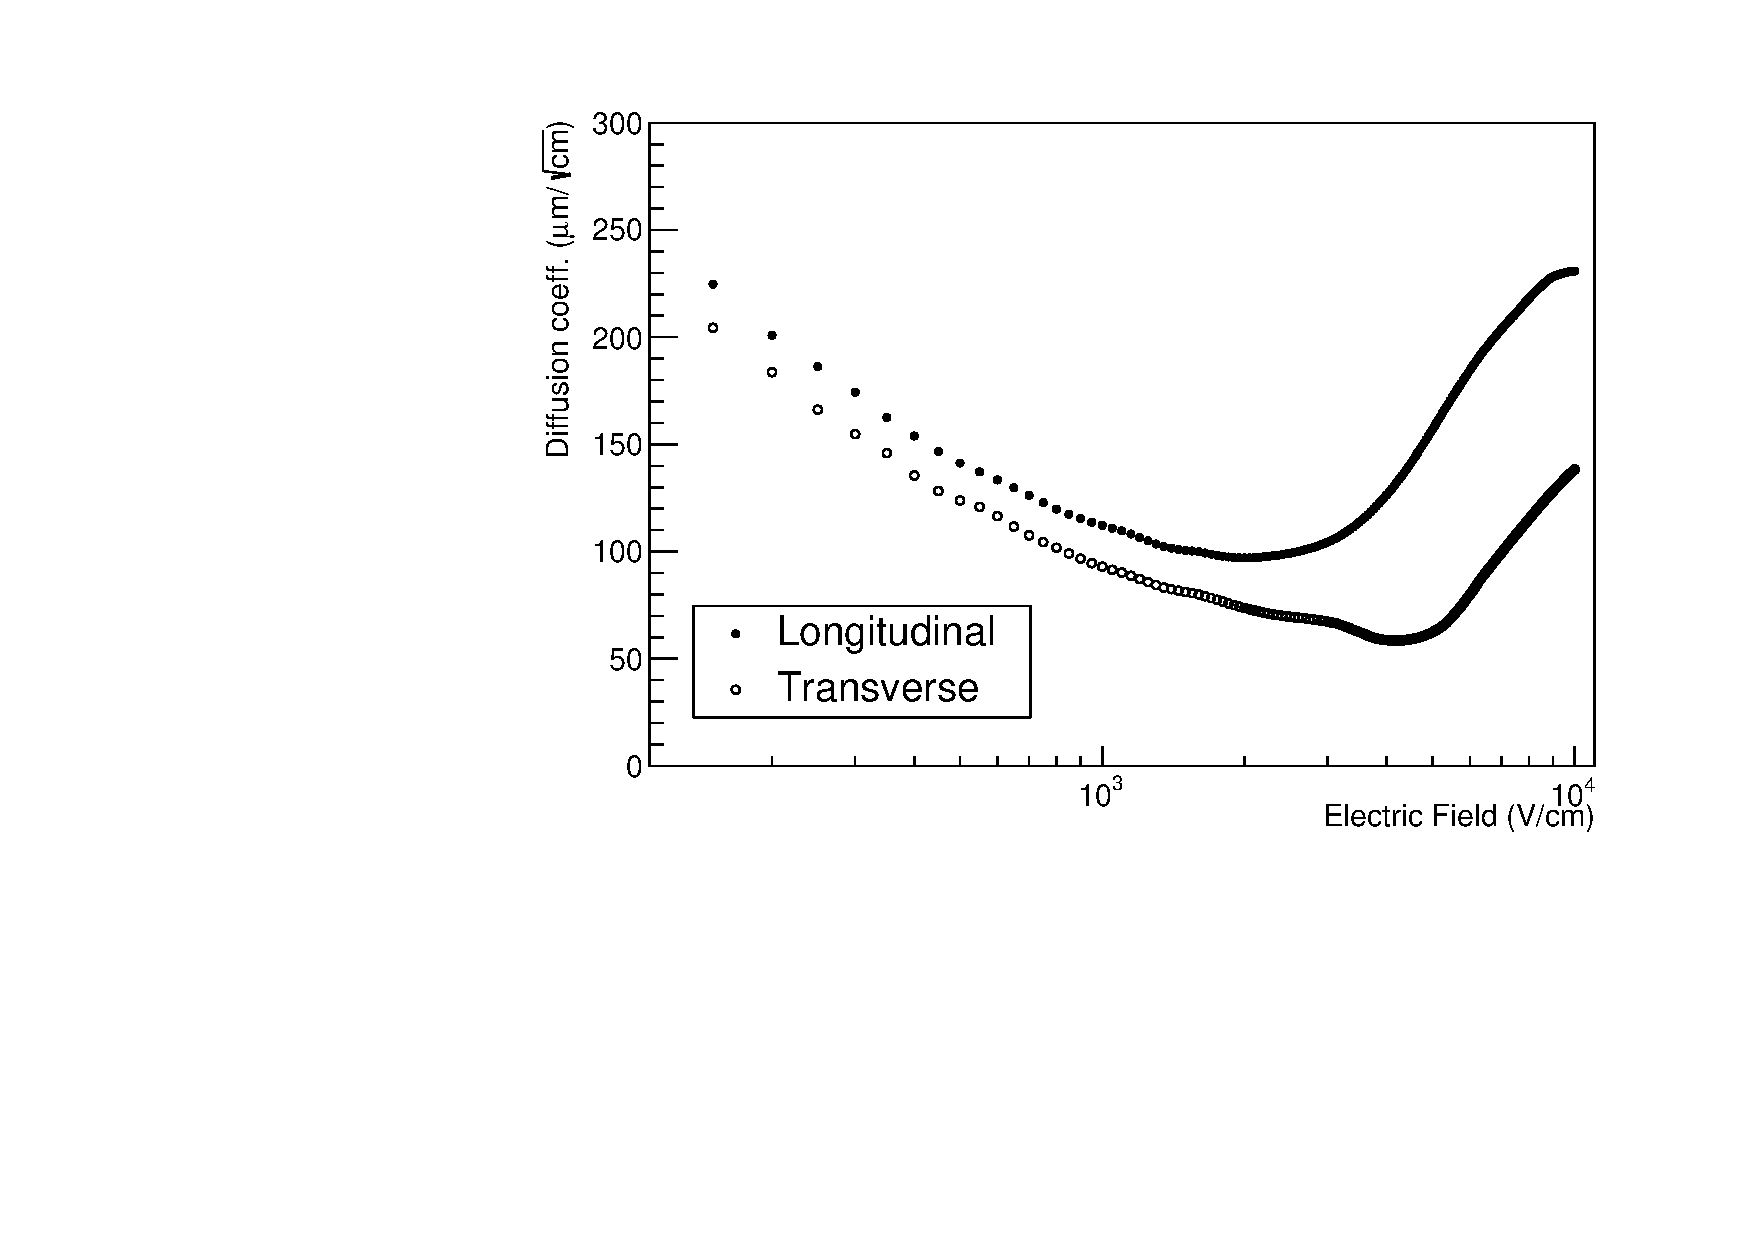
\includegraphics[width=0.4\textwidth]{diff6040.pdf}
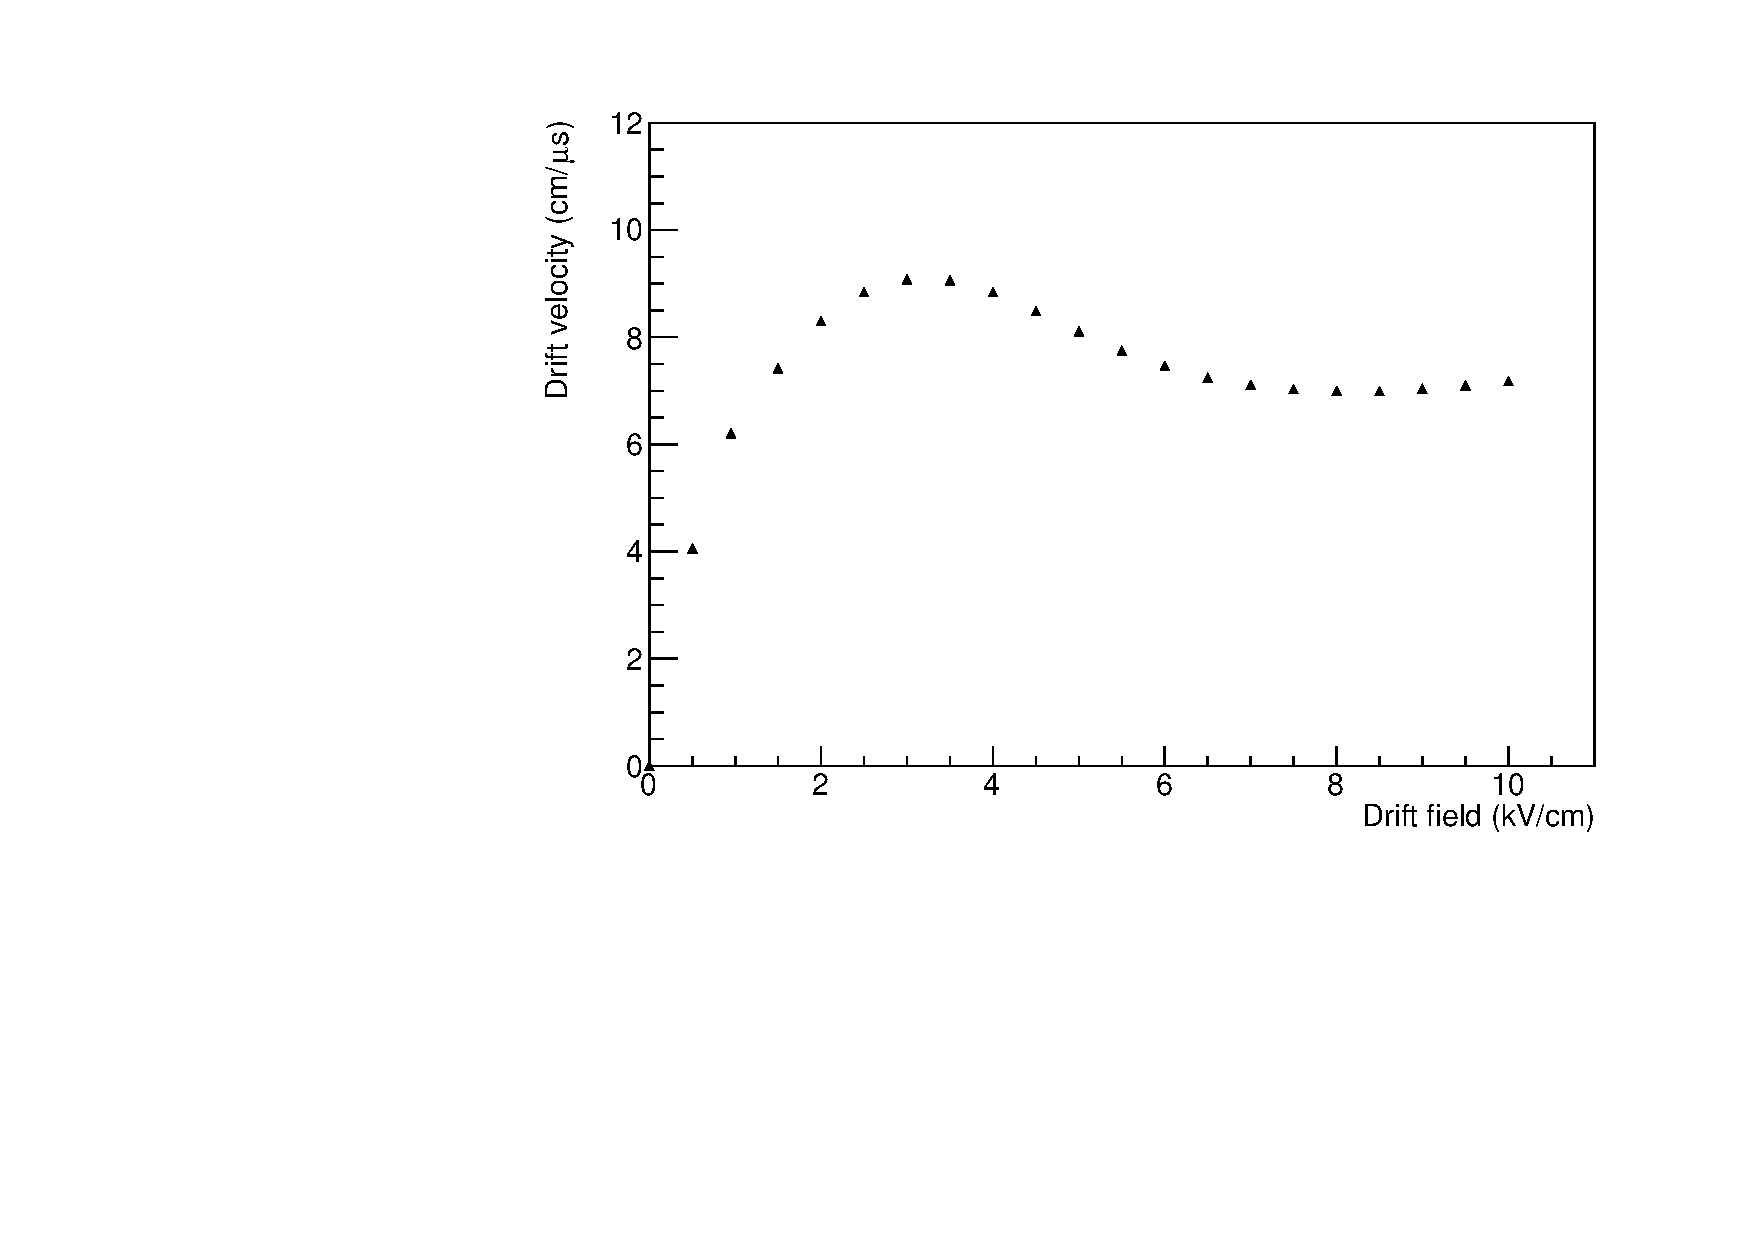
\includegraphics[width=0.4\textwidth]{vdrift6040.pdf}
\caption{Transverse and longitudinal diffusion coefficients (left) and electron drift velocity (right) as a function of the electric field.}
\label{fig:diff_vdrift}
\end{figure}

 A gas mixture with a large fraction of a "cold gas" as the CF$_4$ allows to have a small electron diffusion and quite high drift velocities for electric fields below 1 kV/cm.
 
 Effective ranges of electron and He-nuclei recoils were calculated
respectively by \GEANTfour~\cite{bib:geant} and
\SRIM~\cite{bib:srim}. Results as a function of particle kinetic
energy are shown in Fig.~\ref{fig:range}:
\begin{itemize}
    \item He-nuclei recoils have a sub-millimetre range up to energies
      of 100\keV and are thus expected to produce bright spots with
      sizes mainly dominated by diffusion effects;
    \item low energy (less than 10\keV) electron recoils are in
      general larger then He-nuclei recoils with same energy and are
      expected produce less intense spot-like signals. For a kinetic
      energy of 10\keV, the electron range becomes longer than
      1\unit{mm} and for few tens of \keV, tracks of few centimetres
      are expected.
\end{itemize}

\begin{figure}[ht]
  \begin{center}
    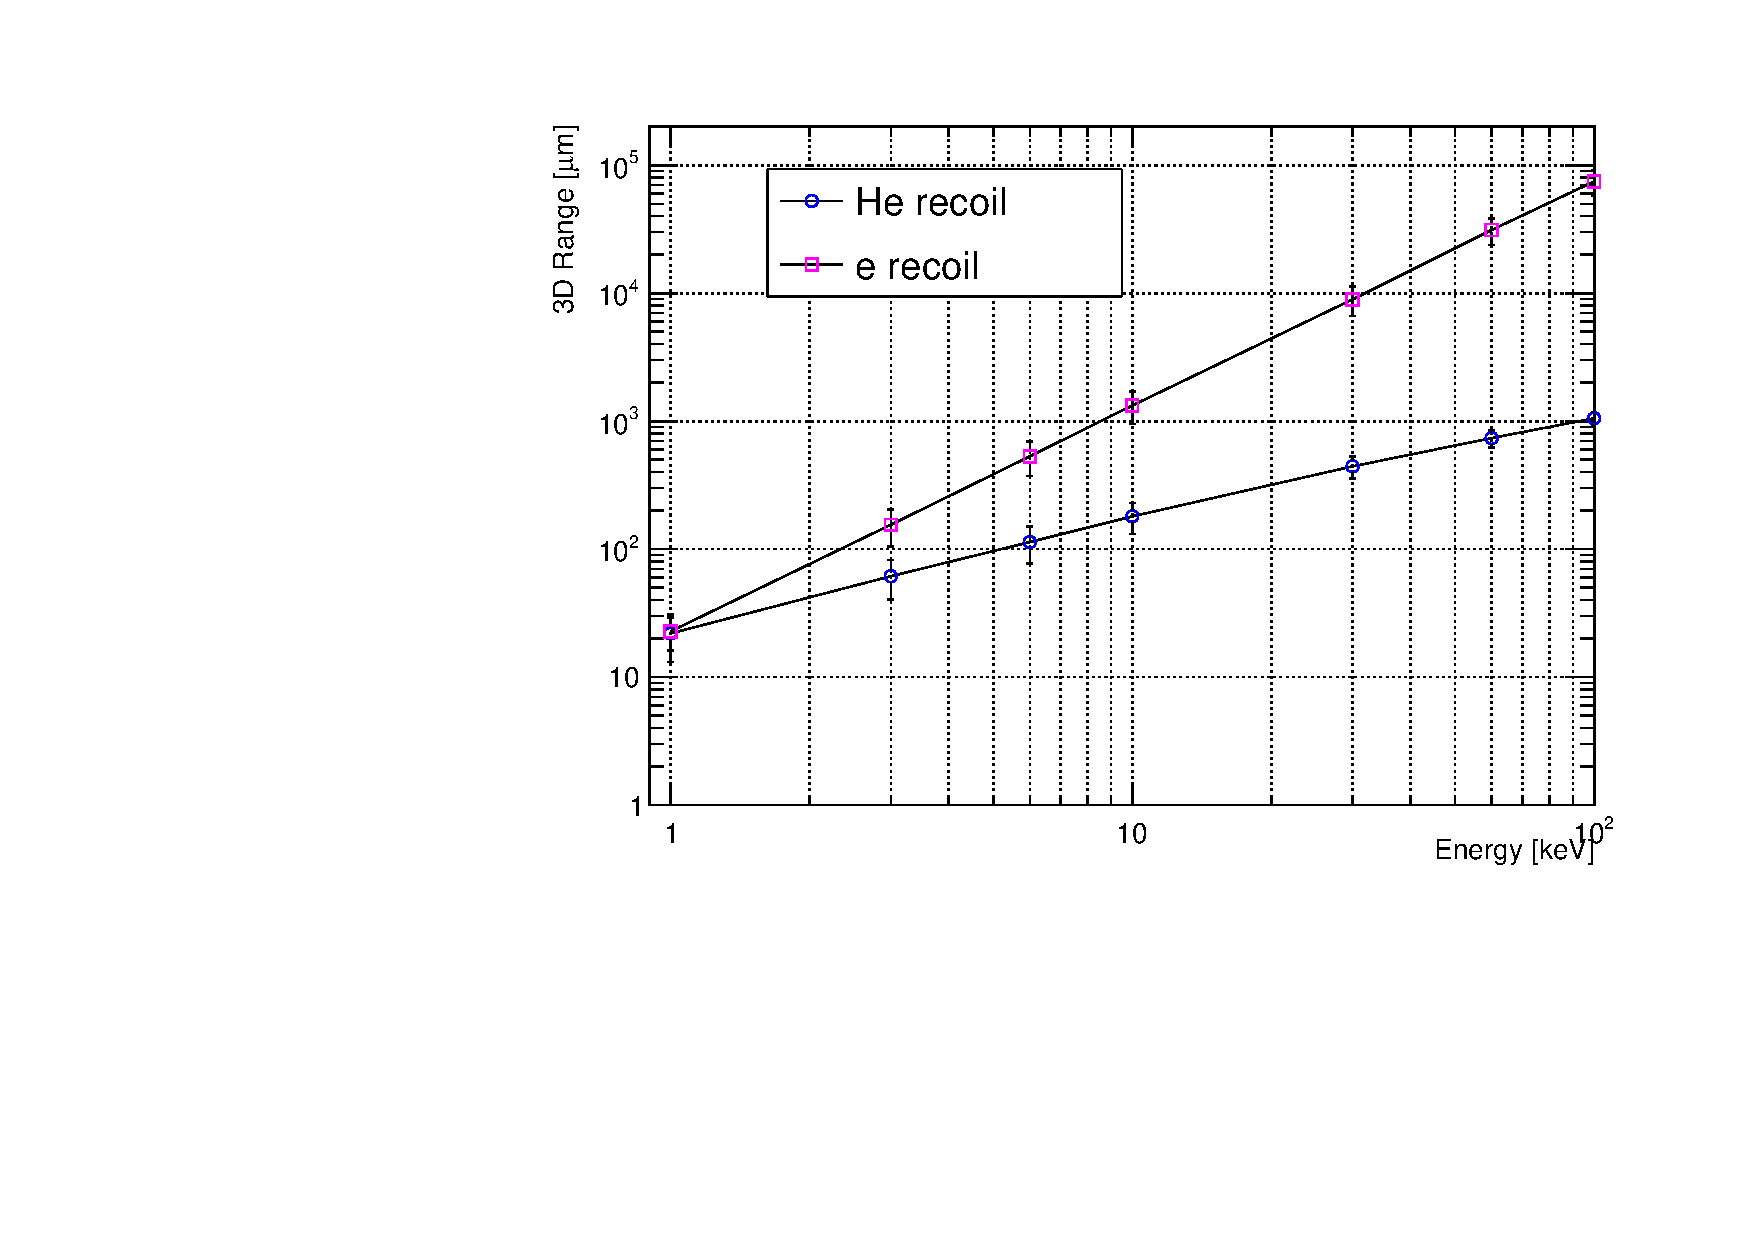
\includegraphics[width=0.49\linewidth]{range_ER_NR.pdf}
    \caption{Average projected ranges for electron and He-nuclei recoils as a faction of their kinetic energy.}
      \label{fig:range}
      \end{center}
\end{figure}


 
\subsection{Sensors}
\label{sect:sensors}

In order to perform a 3D track reconstruction, the profile of the electron
arrival times on the GEM should be acquired.

The main limitation of high granularity CMOS sensors is 
represented by their poor timing information. The maximum possible readout rate of the order of 1 kHz would not allow to have a "time-stamping" better than 1 ms.

To overcome this limitation, CYGNO collaboration proposed and developed the idea of combining the slow sCMOS camera with fast light sensors (PMT os SiPM).
Performance of the combined light readout were tested with the use of a fast PMT \cite{bib:combined} and it was possible to evaluate a resolution on the reconstructed relative {\it z} coordinate of charge clusters of about 100 $\mu$m.

\subsubsection{sCMOS-based Cameras}

As anticipated in Sect.\ref{sect:opro}, high quality cameras are a crucial ingredient for the experiment results. Different cameras were tested during the R\&D phases~\cite{bib:cameras}. All results shown in the paper were obtained by means of the 
 an ORCA Flash 4.0 camera\footnote{For more details visit www.hamamatsu.com}. This device in based on a 1.33~$\times$~1.33~cm$^2$ scientific CMOS sensor, subdivided in 2048~$\times$~2048 pixels with an active area of 6.5~$\times$~6.5~$\mu$m$^2$ each, with
 a quantum efficiency of 70\% at 600~nm and a readout noise of 1.4~electrons.
 The response and noise level of this sensor were tested with a calibrated light source \cite{bib:jinst_orange1}. A response of 0.9 counts/photon was measured together with a pedestal fluctuation of the pedestal of 1.3 photons/pixel. 
 
 This sensor was usually equipped with a Schneider lens with 25~mm focal length $f$ and 0.95 aperture $a$. The lens was placed at the distance $d$ necessary to make the acquisition of the whole GEM surface possible. 
 The geometrical acceptance $\Omega$ can be evaluated as~\cite{bib:ieee_orange}:
$$
 \Omega = \frac{1}{\left(4(\delta+1)\times a \right)^2}
$$

being $\delta = d/f - 1$ the optical de-magnification.

CYGNO apparatus will be equipped with the latest generation sCMOS-based ORCA-Fusion Digital Camera\footnote{https://www.hamamatsu.com/eu/en/product/type/C14440-20UP/index.html} featuring 2304~$times$~2304 pixels with dimensions of $6.5~\times~6.5~\mu$m$^2$, providing a quantum efficiency of 80\% at 600~nm and a readout noise of 0.7~electrons.

\subsubsection{Fast light-sensors}

The information provided by a fast light sensor will be exploited to reconstruct the signal time development and, therefore, its projection on the axis orthogonal to the GEM plane. Different PMT and SiPMT were tested during the R&D phase to individuate the most appropriate in terms of sensitivity and time resolution.

Results presented here were obtained with a
Photonics XP3392 Photo Multiplier Tube (PMT) with a 5~ns rise-time, a maximum QE for 420~nm and a 76~mm square-window.


\section{Experimental Results}
\subsection{\lemon Prototype}
All results reported in this paper were obtained with the Long Elliptical MOdule \lemon. This detector (Fig.~\ref{fig:lemon} is a TPC with a sensitive volume of 7 litres (A) contained in a 20~cm long cylindrical field cage (FC). The base of the cylinder is an ellipse with 24~cm and 20~cm axes. The shape of the FC was chosen in order to couple it with a 24$\times$20~cm$^2$ triple-GEM stack, that closes the sensitive volume on  one side. On the other side, the volume is close be a mesh-based semitransparent cathode. Light produced inside the GEM holes during the multiplication processes is acquired on the GEM side by the ORCA Flash 4.0 camera, and, on the cathode side by the Photonics XP3392 photo-multiplier (Sect. \ref{sect:sensors}.

\begin{figure}[ht]
\centering
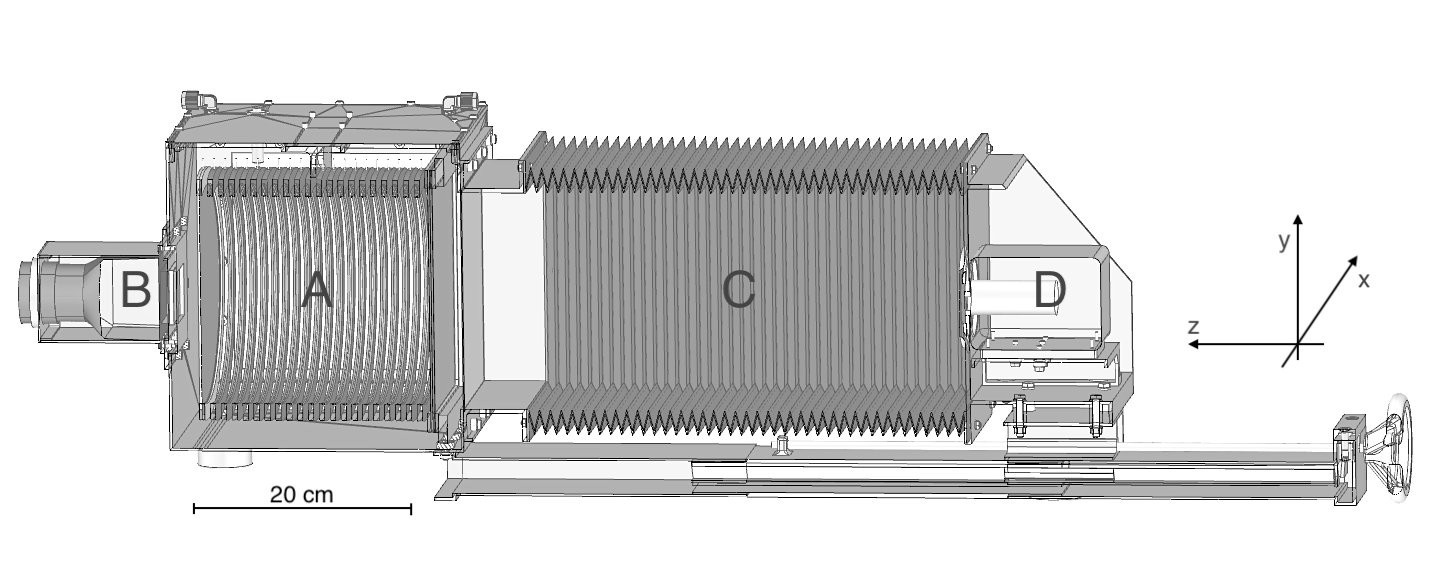
\includegraphics[width=0.9\textwidth]{lemon.png}
\caption{Drawing of the experimental setup. In particular, the elliptical field cage closed on one side by the triple-GEM structure and on the other side by the semitransparent cathode (A), the PMT (B), the adaptable bellow (C) and the CMOS camera with its lens (D) are visible.} \label{fig:lemon}
\end{figure}

The drift volume was filled with He/CF$_4$ based gas mixtures. 


Even if at the beginning they scanned to optimise them, the typical operating configuration for \lemon was based on following sets: 
\begin{itemize}
    \item a gas flux of 200 cc/min;
    \item an electric field within the sensitive volume \Ed~=~0.5~kV/cm;
    \item an electric field in the 2~mm wide gaps between the GEMs \Et~= 2.5~kV/cm;
    \item a voltage difference across the two sides of each GEM \Vg~=~460~V;
\end{itemize}

According to results presented in \cite{bib:roby}, in this configuration an electron gain of about 1.5$\times 10^6$ is expected.

\subsection{Performance Studies}

Performance of \lemon were tested in recent years in laboratory by means of radioactive sources (\fe,\ambe), high energy (400 MeV) electrons from a beam at the BTF facility \cite{bib:btf1,bib:btf2} and cosmic rays.

\subsubsection{Operation Stability}

Detector operational stability was evaluated during a month long test~\cite{bib:fe55New}. 
During the whole period the behavior of all currents drawn by the high voltage channels supplying the electrodes of the GEM stack were monitored and recorded.
In particular, from the correlated analysis of \Ig and images continuously acquired, two different phenomena of electrical instability were observed:

\begin{itemize}
\item {\bf Hot spots.} Appearance of tiny luminous spots (less than 1~mm$^2$ on the GEM surface initially accompanied with a negligible current increase.

These spots could disappear with time or start to slowly grow up (on a time scale of minutes). At some point they could even involve a currents of the order of tens of nano-amperes.

\item{\bf Discharges} High charge density due to very high ionizing particles or charge accumulation on electrode imperfections can suddenly discharge across GEM channels. In these events, a sudden increase in the drawn current is recorded with a voltage restoring on the electrodes through protection resistors on a few seconds time basis. Also these events trigger the recovery procedure.
Even if these events are less frequent than hot spots 
they can be dangerous for the GEM structure and the energy released in the discharge can, in principle, damage it.

\end{itemize}

A completely automatic high voltage control and recovery procedure was developed. In case of drawn currents larger than a certain threshold all \Vg\ are decreased of 100~V and then slowly restored in about 3~minutes.

From the monitoring of detector current it resulted an occurrence probability of about 10 hot-spots/day and 6 discharges/day.
A detailed analysis of the time distance between two of these phenomena didn't shown any correlation between two subsequent events neither any increase of their rates. This allowed to conclude than
detector operation looked very safe and stable and the provided performance was completely satisfactory. 

The instability events gave rise to a detection inefficiency due to dead time introduced by recovering procedures of less than 4\%.

Other gas proportion were tested and it resulted evident that a lower amount of CF$_4$, able to quench and avoid large charge productions gave a less stable electrostatic configuration. 

\subsubsection{Light Yield and Energy Resolution}

The light production was evaluated by analysing sCMOS and PMT response for interactions in gas of 5.9~keV produced by a \fe source.

Figure~\ref{fig:light} shows the spectra of the amount of light detected in spots reconstructed on sCMOS sensor.

\begin{figure}[ht]
\centering
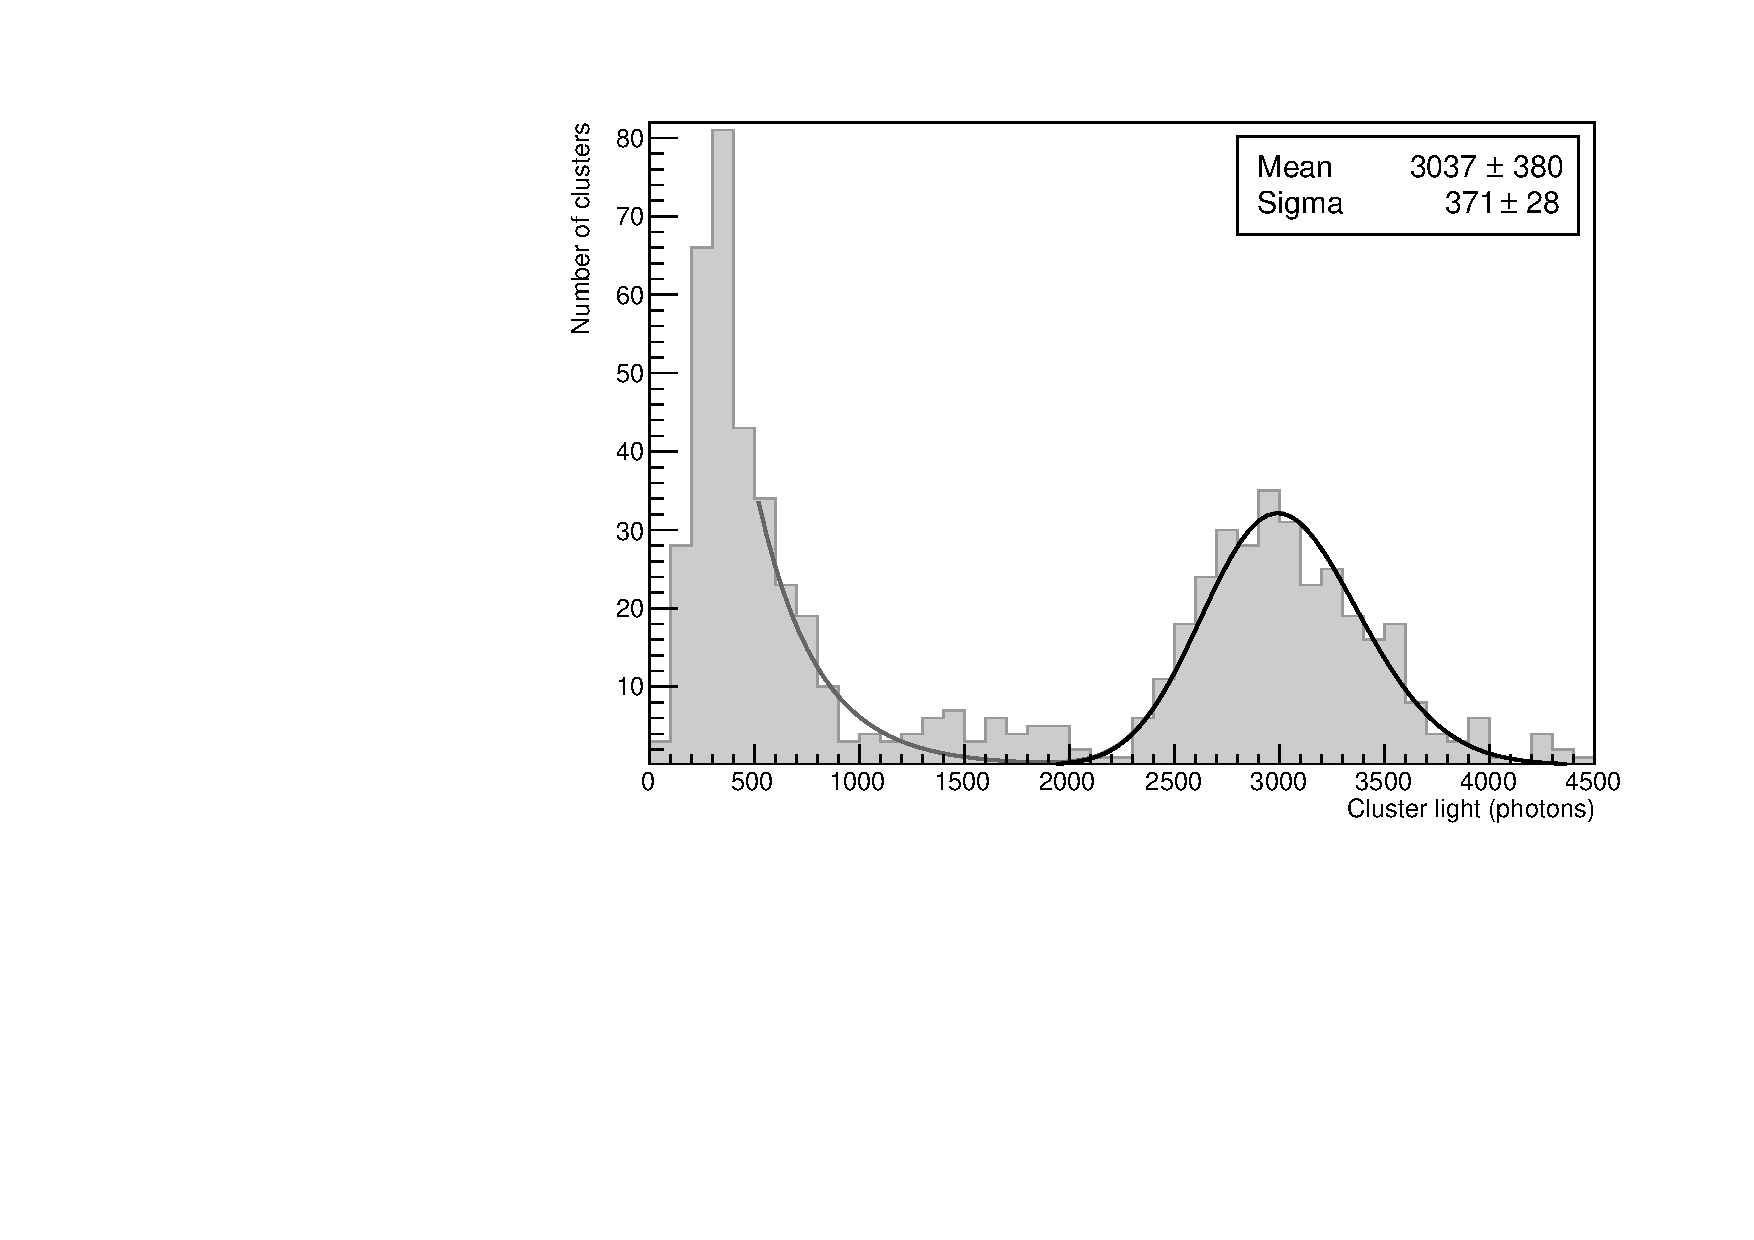
\includegraphics[width=0.45\textwidth]{DB_Integral_6040.pdf}
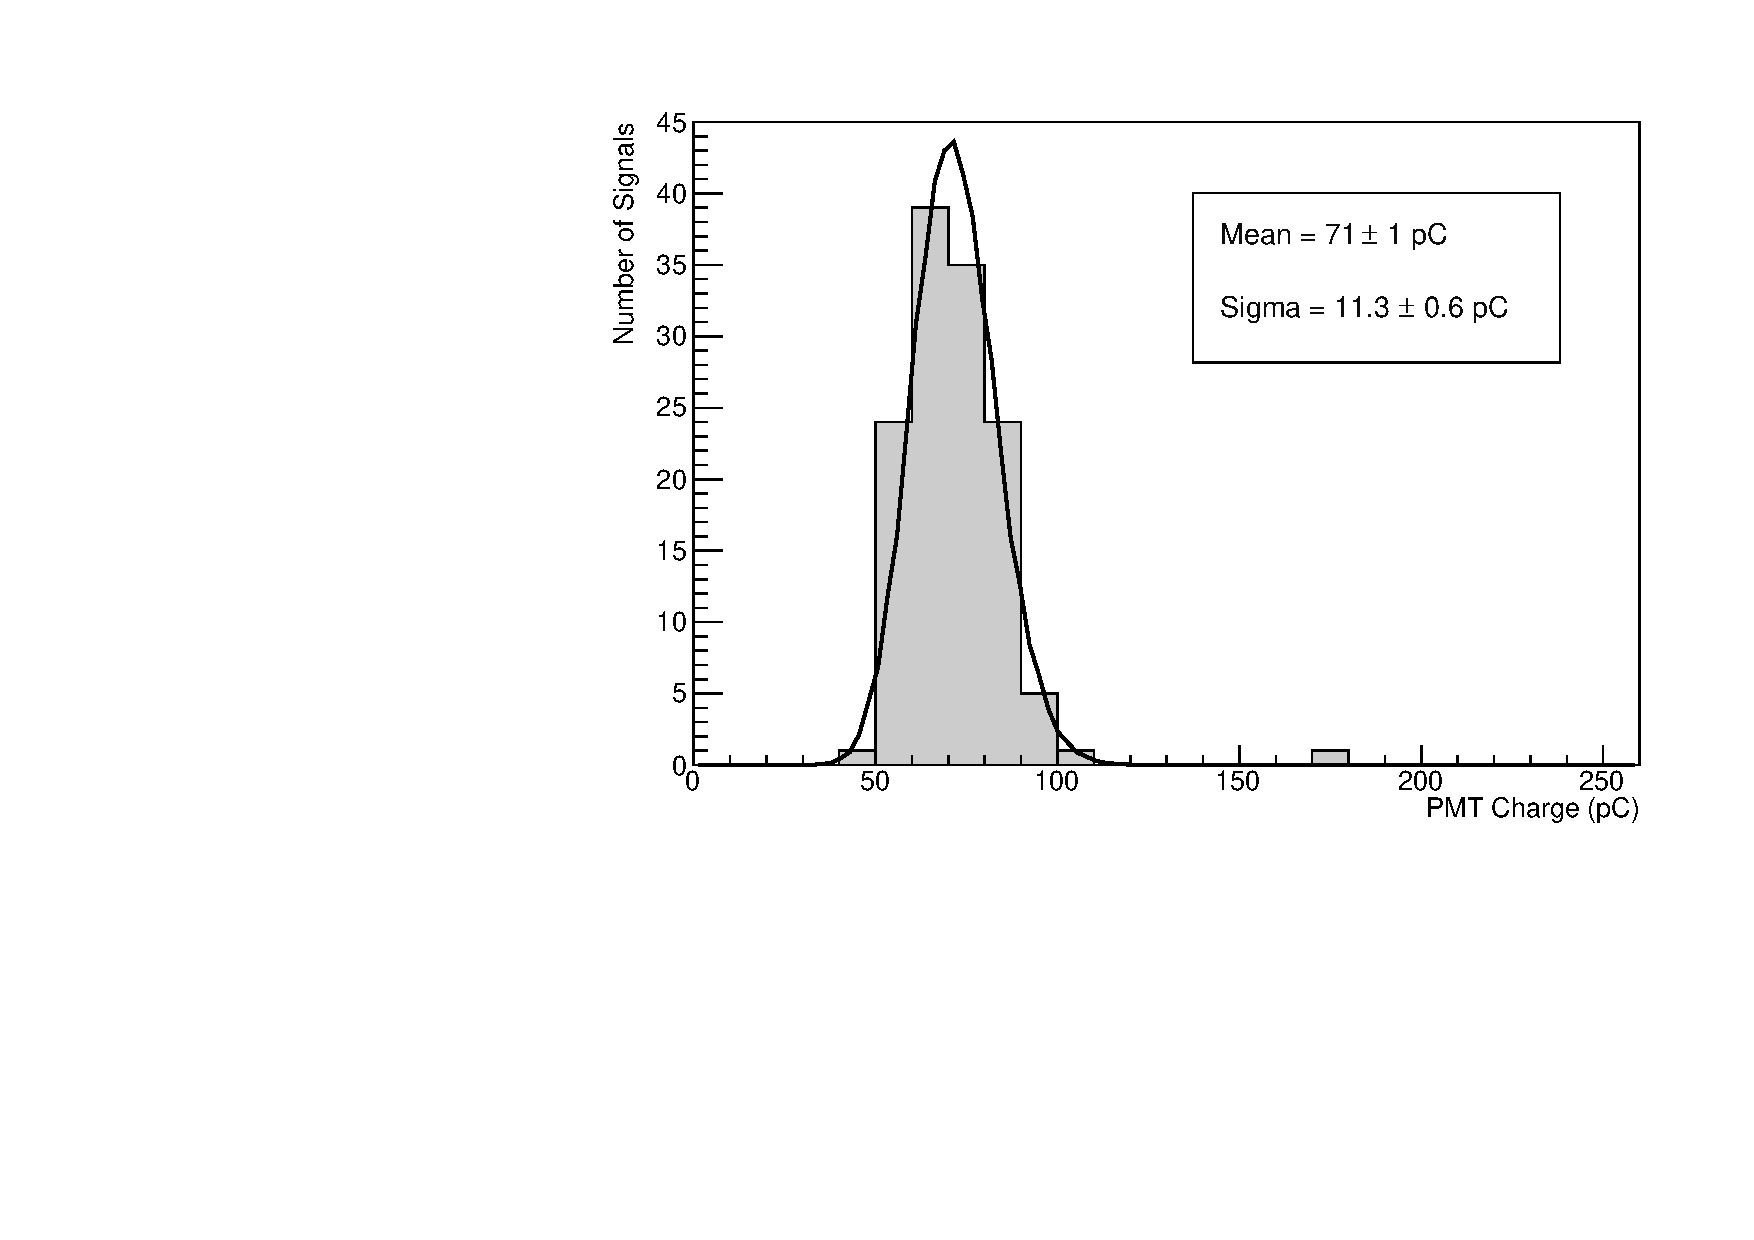
\includegraphics[width=0.45\textwidth]{newlightCharge_Run1834_Mix60-40.pdf}
\caption{Distribution of the light content in spots (left) and distribution of the charge provided by the PMT (right).} 
\label{fig:light}
\end{figure}

Average light yields for the two mixtures were evaluated from a Polya fit \cite{bib:rolandiblum} to the two distributions:
\begin{itemize}
    \item sCSMOS provides an average value of 514~$\pm$~63 detected photons per keV released in the gas (in agreement with results obtained with lower \Vg\ and \Et\ \cite{bib:fe55}) with an energy resolution of 12.2\%;
    \item PMT provides an average value of (12.0~$\pm$~0.2) pC per keV released in the gas with an energy resolution of 15.5\%;

\end{itemize}


The similar energy resolution provided by the two gas mixture indicates that the main contribution to this parameter is due the fluctuations of electron multiplication processes.


\subsubsection{Detection Efficiency}

The capability of detecting low energy spots in the sensitive volume was tested by exploiting photons emitted by \fe source.
Figure \ref{fig:deteff} shows, on the left, the behavior of the number $n$ of reconstructed spots as a function of electric field in the drift volume normalized to the value obtained for \Ed~=~600~V/cm.
The plateau found for \Ed\ values larger than 300~V/cm indicates that starting from that value, a full detection efficiency is found. 
On the right of Fig.~\ref{fig:deteff} the behavior of $n$ as a function of spot distance from the GEM plane (right) normalised to its average value $\overline{n}$ is shown.

\begin{figure}[ht]
\centering
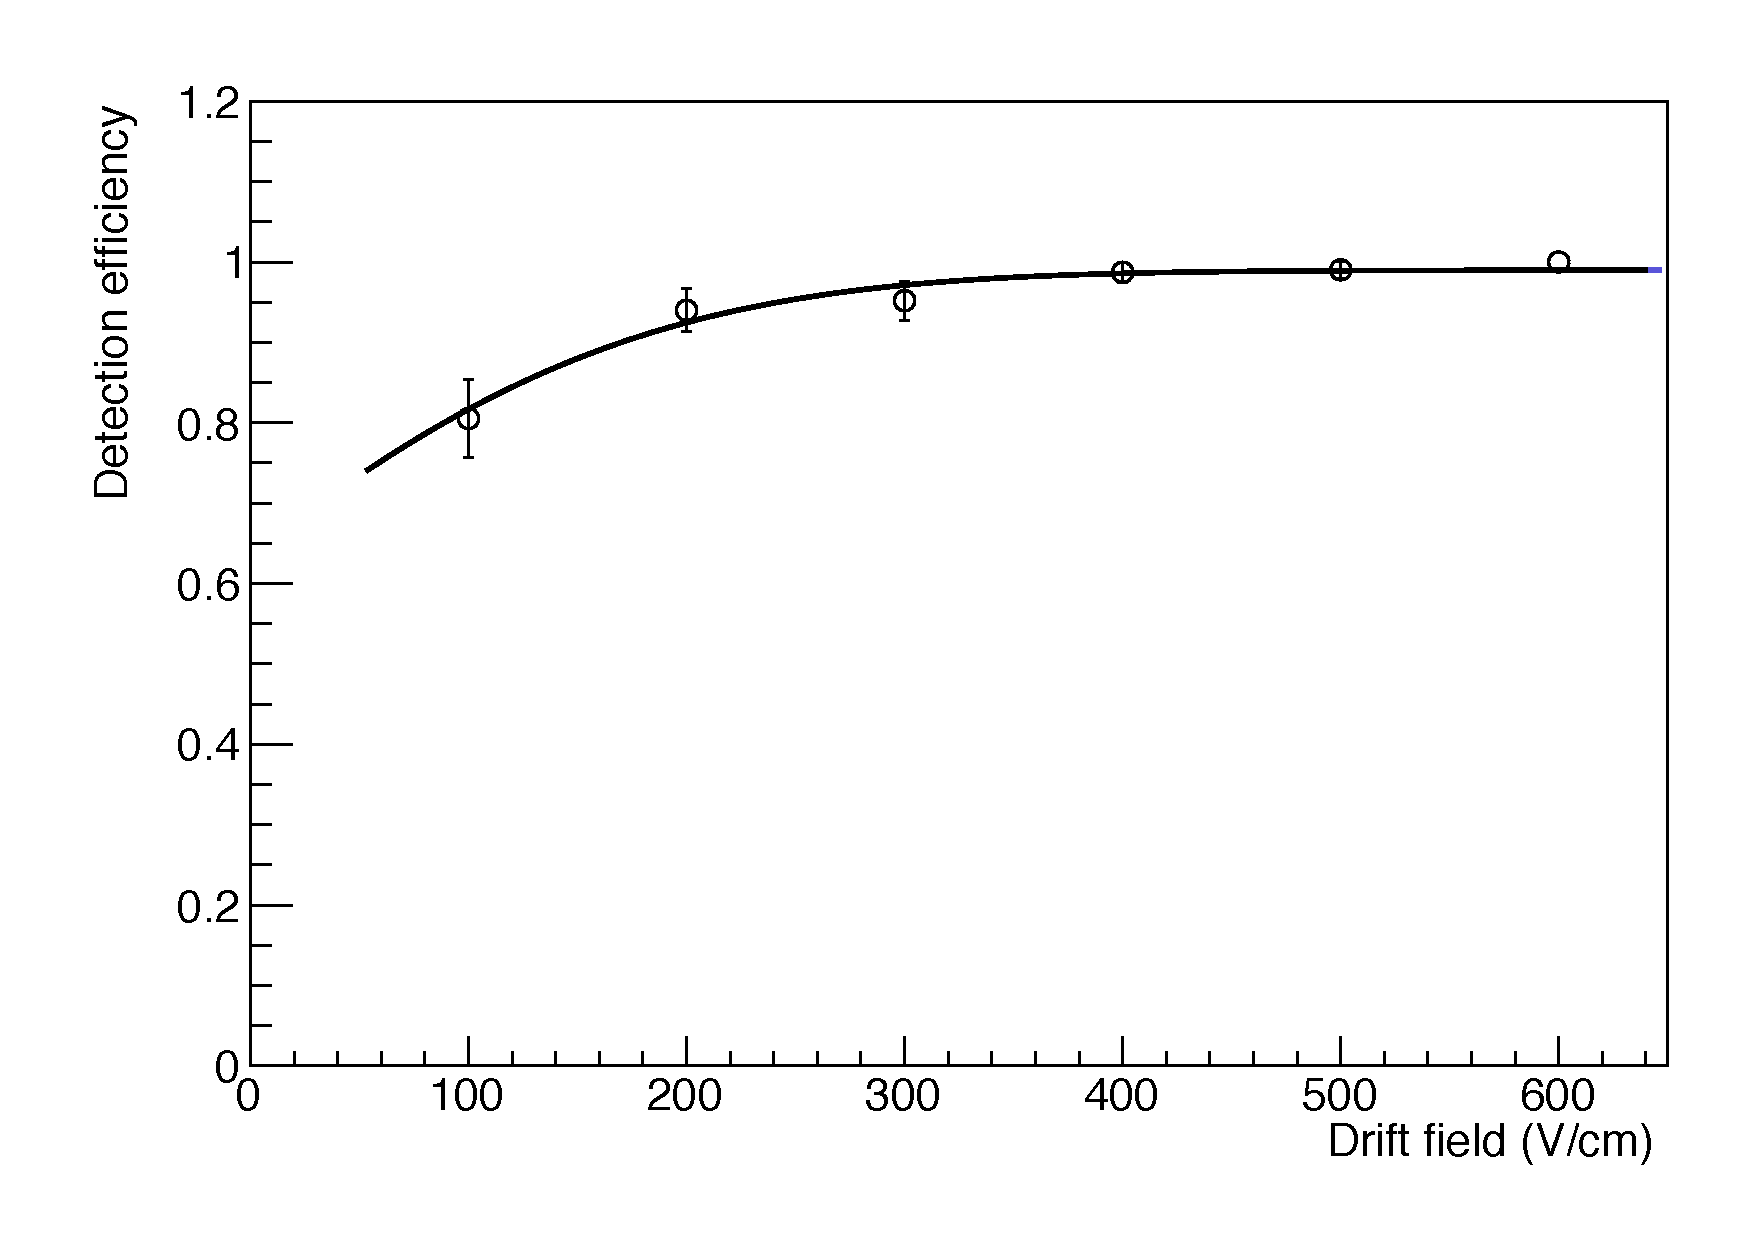
\includegraphics[width=0.45\textwidth]{gEff_Edrift.pdf}
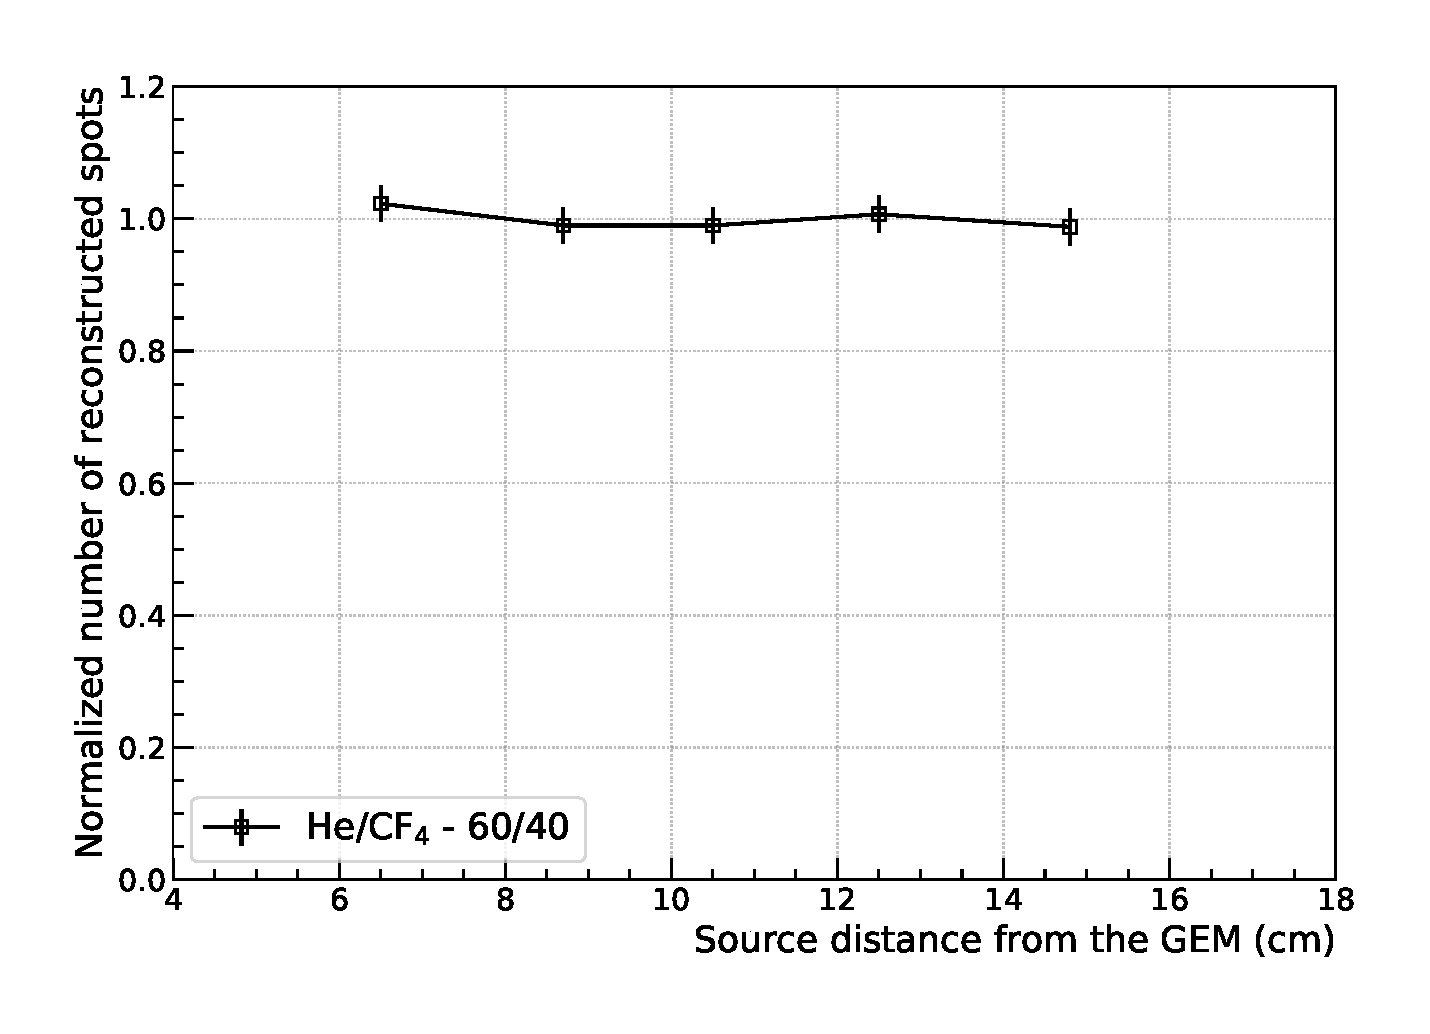
\includegraphics[width=0.45\textwidth]{feZscan6040_wo_4.pdf}
\caption{Behavior of the normalized number of \fe spots as a function of drift electric field (left) and event depth in sensitive volume (right).} 
\label{fig:deteff}
\end{figure}

A constant behavior was found in all tested positions allowing to conclude that no evidences of inefficiency in event detection were found.

\subsubsection{Tracking Performance}

High energy particles crossing the detector can give rise to tracks several
centimetre long.
This can be the case for muons from cosmic rays of electron recoils with energies of about 100~keV or more. 
Performance in reconstructing long track were studied at the Beam Test Facility (BTF) of "Laboratori Nazionali di Frascati" \cite{bib:btf1,bib:btf2}
Reults are described in details in \cite{bib:ieee17, bib:ieee18, bib:lemon_btf}. They indicate that track segments with lengths lower than 1~cm can be reconstructed with a resolution on relative position between 100~$\mu$m (near the GEM plane) and 300~$\mu$m (20~cm~far from GEM plane).
Moreover, by exploiting the diffusion effect in gas, the distance of each of those segments can be evaluated, separately by the CMOS sensor and PMT, with a precision between 10\% and 20\%.

\section{Detection and Identification of Nuclear Recoils}



\section{Detection and Identification of Electron Recoils}

\section{The CYGNO Apparatus}

\subsection{Detector Description}
\subsection{Background Simulation}

\begin{table}[h!]
\centering
\caption{Background rates. Copper costs (25 \EUR{}/kg) assuming for LIME: $50\times50\times100$~cm$^3$ internal shielding size; 0.162~m$^3$ for 5~cm, 0.406~m$^3$ for 10~cm, 1.188~m$^3$ for 20~cm; 
for 4$\times$LIME: $90\times90\times200$~cm$^3$ internal shielding size 1.040~m$^3$ for 10~cm}
\begin{tabular}{|c|c|c|c|c|} 
 \hline
Detector        & Water/Copper   & Water         &  Copper & [1-20]~keV \\
Volume (m$^3$)  & Thickness (cm) & Cost (k\EUR{})&  Cost (k\EUR{}) & cpy    \\
\hline
\hline
%1 & - & - & 1  & & & 1 $\times 10^{10}$ \\
%\hline
1 & 250/5 & & & 1 $\times 10^{2}$ \\
\hline
1 & 200/5 & & & 1 $\times 10^{3}$ \\
\hline
1 & 100/5 & & & 2 $\times 10^{5}$ \\
\hline
1 & 85/5 & & & 1 $\times 10^{6}$ \\
\hline
1 & 50/5 & & & 8 $\times 10^{6}$ \\
\hline
\hline
0.05 & - & - & - & 3$\times 10^8$ \\
\hline
0.05 & 50/5 & 20 & 40 & 5$\times 10^5$ \\
\hline
0.05 & 50/10 & 20 & 95 & 5$\times 10^4$ \\
\hline
0.05 & 100/5 & 25 & 40 & 3$\times 10^4$ \\
\hline
0.05 & 110/10 & 25 & 95 & 2$\times 10^3$ \\
\hline
0.05 & 50/20 & 20 & 270 & 1$\times 10^3$ \\
\hline
0.40 & 90/10 & 50 & 250 & 2$\times 10^4$ \\
\hline
\hline
\end{tabular}
\label{tab:shield}
\end{table}


\section{Physics Performance}
\section*{References}

\bibliography{cygno}

\end{document}